\documentclass[11pt,a4paper]{article}

\usepackage[utf8]{inputenc}
\usepackage[T1]{fontenc}
\usepackage{mathpazo}
\usepackage[scaled=0.92]{helvet}
\usepackage[margin=1in]{geometry}
\usepackage{graphicx}
\usepackage{amsmath,amssymb,amsfonts}
\usepackage{booktabs}
\usepackage{tabularx}
\usepackage{setspace}
\usepackage{titlesec}
\usepackage{fancyhdr}
\usepackage{float}
\usepackage{caption}
\usepackage{microtype}
\usepackage{tikz}
\usepackage{xcolor}
\usepackage{listings}
\usepackage[hidelinks]{hyperref}

\usetikzlibrary{shapes.geometric, arrows.meta, positioning, calc, matrix, fit, backgrounds}

\setstretch{1.15}
\setlength{\parindent}{0pt}
\setlength{\parskip}{0.8em}
\sloppy

\titleformat{\section}{\normalfont\large\bfseries\sffamily}{\thesection}{1em}{}
\titleformat{\subsection}{\normalfont\normalsize\bfseries\sffamily}{\thesubsection}{1em}{}
\titleformat{\subsubsection}{\normalfont\normalsize\itshape\sffamily}{\thesubsubsection}{1em}{}

\pagestyle{fancy}
\fancyhf{}
\fancyhead[L]{\small\sffamily Teori Himpunan untuk RPL}
\fancyhead[R]{\small\sffamily\thepage}
\renewcommand{\headrulewidth}{0.4pt}

\captionsetup{font=small,labelfont=bf,labelsep=period}

\renewenvironment{abstract}
{\small
	\begin{center}\textbf{\sffamily Abstrak}\end{center}
	\begin{quote}}
	{\end{quote}}

\lstdefinestyle{code}{
	basicstyle=\ttfamily\small,
	frame=single,
	rulecolor=\color{black},
	breaklines=true,
	showstringspaces=false,
	columns=fullflexible,
	keepspaces=true,
	framesep=6pt,
	aboveskip=1em,
	belowskip=1em,
	xleftmargin=0pt
}

\lstdefinestyle{out}{
	basicstyle=\ttfamily\small,
	frame=tb,
	rulecolor=\color{black},
	breaklines=true,
	showstringspaces=false,
	columns=fullflexible,
	keepspaces=true,
	framesep=4pt,
	aboveskip=1em,
	belowskip=1em
}

\title{\vspace{-1.5cm}\textbf{\sffamily\LARGE Teori Himpunan untuk Rekayasa Perangkat Lunak\\ Modul Pembelajaran dengan Visualisasi Presisi}}
\author{
	\textbf{Muhammad Riduwan Khafidi} \\
	\small Program Studi Teknik Rekayasa Perangkat Lunak \\
	\small Politeknik Negeri Batam \\
	\small \texttt{4342611034@students.polibatam.ac.id}
}
\date{\small\today}

\begin{document}

\maketitle
\thispagestyle{empty}

\begin{abstract}
	Modul ini menjelaskan teori himpunan sebagai alat pemodelan data dan logika dalam rekayasa perangkat lunak. Pembahasan dimulai dari definisi, penyajian, kardinalitas, himpunan khusus, operasi himpunan, prinsip inklusi-eksklusi, hingga himpunan fuzzy. Setiap konsep disertai alasan mengapa diperlukan, langkah kerja, contoh terapan, dan deskripsi tekstual untuk pembaca yang mengandalkan narasi. Modul ini memuat sepuluh visualisasi TikZ, sembilan tabel, dan satu studi kasus bertahap tentang dashboard pengguna e-commerce. Melalui modul ini, pembaca memperoleh kerangka dari data mentah menjadi keputusan yang dapat dihitung dan dipertanggungjawabkan.
\end{abstract}

\section{Pendahuluan}

\subsection{Analogi Pembuka}

Bayangkan sebuah gudang arsip dengan banyak lemari. Setiap lemari diberi label, setiap laci diberi nomor, dan setiap dokumen hanya boleh masuk ke satu laci yang benar. Jika dokumen yang sama dimasukkan ke tiga laci berbeda, pencarian menjadi lambat dan laporan menjadi salah. Teori himpunan bekerja seperti aturan lemari arsip itu: ia menentukan apa yang termasuk, apa yang tidak termasuk, dan bagaimana kumpulan yang berbeda digabungkan atau dipisahkan.

\subsection{Mengapa Topik Ini Penting}

Sistem perangkat lunak menyimpan data sebagai kumpulan objek yang harus unik. Daftar pengguna, daftar produk, daftar transaksi, dan daftar hak akses adalah himpunan. Tanpa teori himpunan, seorang pengembang sulit menjawab pertanyaan seperti berapa pengguna unik, siapa yang memakai dua platform sekaligus, dan mengapa jumlah pelanggan tidak boleh dihitung dengan menjumlahkan semua kategori secara langsung. Teori himpunan memberi bahasa yang presisi untuk menjawab pertanyaan itu.

\subsection{Peta Pembahasan}

Bagian kedua membahas konsep dasar himpunan. Bagian ketiga membahas himpunan khusus dan relasi antar himpunan. Bagian keempat membahas operasi himpunan. Bagian kelima membahas prinsip inklusi-eksklusi. Bagian keenam membahas himpunan fuzzy. Bagian ketujuh menyandingkan seluruh konsep. Bagian kedelapan memakai konsep itu pada studi kasus dashboard pengguna. Bagian kesembilan dan kesepuluh memberi daftar kesalahan umum dan lembar rujukan cepat.

\section{Konsep Dasar Himpunan}

\subsection{Definisi dan Notasi}

Himpunan adalah kumpulan objek berbeda yang terdefinisi dengan jelas. Objek di dalam himpunan disebut elemen. Notasi himpunan memakai kurung kurawal. Jika $U$ adalah himpunan pengguna unik, maka penulisan $U=\{\text{USR01},\text{USR02},\text{USR03}\}$ berarti $U$ berisi tiga pengguna berbeda. Penulisan $x \in U$ berarti $x$ adalah elemen $U$, sedangkan $x \notin U$ berarti $x$ bukan elemen $U$ \cite{rosen}.

Himpunan berbeda dari larik mentah. Larik boleh memuat duplikat, sedangkan himpunan tidak. Larik $[\text{USR01},\text{USR02},\text{USR01}]$ memiliki tiga posisi, tetapi himpunan dari larik itu hanya memiliki dua elemen, yaitu USR01 dan USR02. Perbedaan ini penting dalam basis data karena duplikat membuat hitungan pengguna aktif menjadi terlalu besar. Perhatikan Gambar~\ref{fig:hierarki-data}.

\begin{figure}[H]
	\centering
	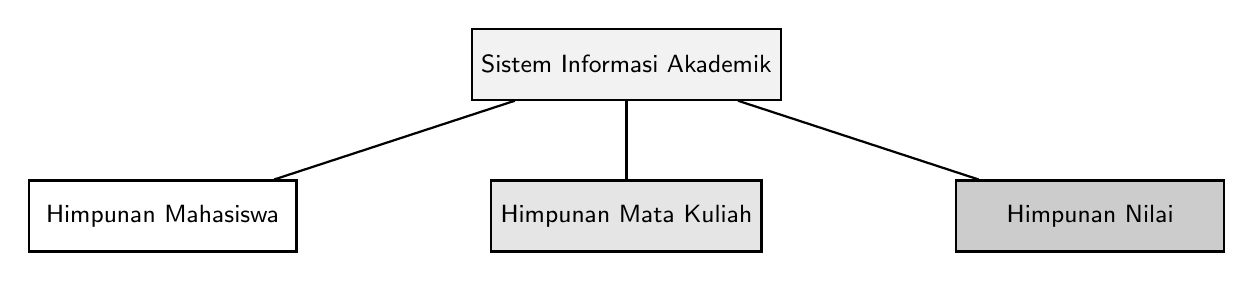
\begin{tikzpicture}[
			node distance=0.5cm and 0.8cm,
			box/.style={rectangle, draw=black, thick, minimum width=3.4cm, minimum height=0.9cm, align=center, font=\sffamily\small},
			line/.style={draw, thick}
		]
		\node[box, fill=black!5] (root) {Sistem Informasi Akademik};
		\node[box, fill=white, below left=1cm and 2.2cm of root] (mhs) {Himpunan Mahasiswa};
		\node[box, fill=black!10, below=1cm of root] (mk) {Himpunan Mata Kuliah};
		\node[box, fill=black!20, below right=1cm and 2.2cm of root] (nilai) {Himpunan Nilai};

		\draw[line] (root) -- (mhs);
		\draw[line] (root) -- (mk);
		\draw[line] (root) -- (nilai);
	\end{tikzpicture}
	\caption{Hierarki data akademik sebagai kumpulan himpunan.}
	\label{fig:hierarki-data}
\end{figure}

Deskripsi tekstual Gambar~\ref{fig:hierarki-data}: satu kotak utama berada di atas, lalu tiga kotak bercabang ke kiri, tengah, dan kanan. Kotak utama adalah sistem informasi akademik. Tiga kotak cabang adalah himpunan mahasiswa, himpunan mata kuliah, dan himpunan nilai. Gradasi abu-abu hanya membedakan tingkat, bukan menyatakan makna warna.

\subsection{Penyajian Himpunan}

Himpunan dapat disajikan dengan empat cara utama. Cara pertama adalah enumerasi, yaitu menuliskan semua elemen. Contoh: $A=\{101,102,105,108,112\}$. Cara kedua adalah simbol baku, misalnya $\mathbb{N}=\{1,2,3,\ldots\}$ untuk bilangan asli. Cara ketiga adalah notasi pembentuk himpunan, misalnya $B=\{x \mid 100 \le x \le 115 \text{ dan } x \text{ habis dibagi } 3\}$. Cara keempat adalah diagram Venn, yaitu gambar daerah yang mewakili himpunan \cite{munir}. Perhatikan Gambar~\ref{fig:empat-penyajian}.

\begin{figure}[H]
	\centering
	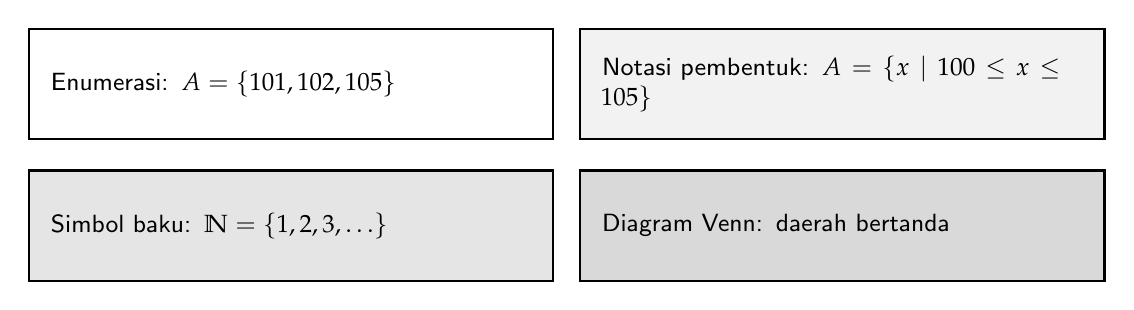
\begin{tikzpicture}[
			box/.style={rectangle, draw=black, thick, text width=6.1cm, minimum height=1.4cm, align=left, font=\sffamily\small, inner sep=8pt}
		]
		\node[box, fill=white] (a) at (0,1.8) {Enumerasi: $A=\{101,102,105\}$};
		\node[box, fill=black!5] (b) at (7,1.8) {Notasi pembentuk: $A=\{x \mid 100 \le x \le 105\}$};
		\node[box, fill=black!10] (c) at (0,0) {Simbol baku: $\mathbb{N}=\{1,2,3,\ldots\}$};
		\node[box, fill=black!15] (d) at (7,0) {Diagram Venn: daerah bertanda};
	\end{tikzpicture}
	\caption{Empat cara menyajikan himpunan.}
	\label{fig:empat-penyajian}
\end{figure}

Deskripsi tekstual Gambar~\ref{fig:empat-penyajian}: empat kotak tersusun dua baris dan dua kolom. Kotak kiri atas berisi enumerasi. Kotak kanan atas berisi notasi pembentuk. Kotak kiri bawah berisi simbol baku bilangan asli. Kotak kanan bawah berisi diagram Venn. Setiap kotak memakai gradasi abu-abu berbeda untuk memisahkan cara penyajian tanpa memakai warna.

\subsection{Kardinalitas}

Kardinalitas adalah banyaknya elemen berbeda dalam himpunan berhingga. Notasinya $|A|$ atau $n(A)$. Jika log mentah berisi $[\text{USR01},\text{USR05},\text{USR02},\text{USR01},\text{USR03},\text{USR05},\text{USR01},\text{USR04},\text{USR02}]$, maka himpunan pengguna uniknya adalah $\{\text{USR01},\text{USR05},\text{USR02},\text{USR03},\text{USR04}\}$. Kardinalitas himpunan itu adalah lima, bukan sembilan, karena empat kemunculan berulang tidak dihitung lagi. Inilah dasar perhitungan pengguna unik dalam sistem analitik \cite{epp}. Ringkasan notasi dasar diberikan pada Tabel~\ref{tab:notasi-dasar}.

\begin{table}[H]
	\centering
	\caption{Ringkasan notasi dasar himpunan.}
	\label{tab:notasi-dasar}
	\small
	\begin{tabularx}{\textwidth}{l X}
		\toprule
		Notasi          & Makna                                     \\
		\midrule
		$x \in A$       & $x$ adalah elemen himpunan $A$            \\
		$x \notin A$    & $x$ bukan elemen himpunan $A$             \\
		$|A|$           & kardinalitas, yaitu banyak elemen berbeda \\
		$A \subseteq B$ & setiap elemen $A$ juga elemen $B$         \\
		$\varnothing$   & himpunan kosong                           \\
		$P(A)$          & himpunan kuasa dari $A$                   \\
		\bottomrule
	\end{tabularx}
\end{table}

\section{Himpunan Khusus dan Relasi Antar Himpunan}

\subsection{Himpunan Kosong dan Subset}

Himpunan kosong adalah himpunan tanpa elemen. Notasinya $\varnothing$ atau $\{\}$. Himpunan $A$ disebut himpunan bagian dari $B$ jika setiap elemen $A$ juga elemen $B$. Notasinya $A \subseteq B$. Contoh: $\{1,2,3\} \subseteq \{1,2,3,4,5\}$. Dalam sistem hak akses, jika Admin memiliki semua hak akses dan Dosen hanya memiliki sebagian, maka himpunan hak akses Dosen adalah subset dari himpunan hak akses Admin \cite{lipschutz}. Perhatikan Gambar~\ref{fig:subset}.

\begin{figure}[H]
	\centering
	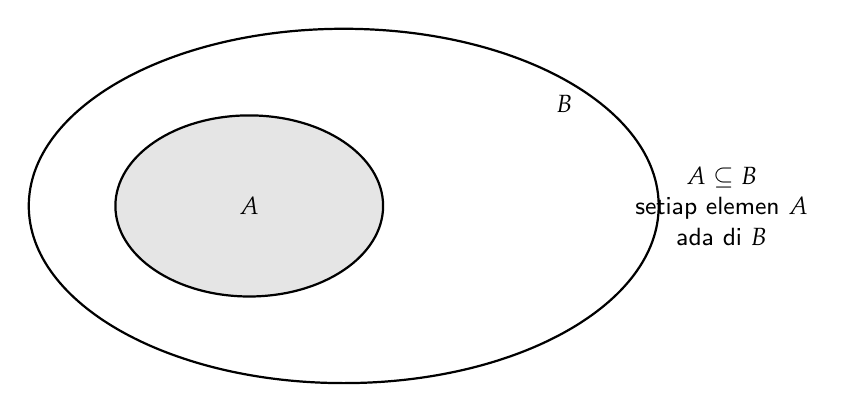
\begin{tikzpicture}[
			set/.style={ellipse, draw=black, thick, minimum width=8cm, minimum height=4.5cm, align=center, font=\sffamily\small},
			sub/.style={ellipse, draw=black, thick, fill=black!10, minimum width=3.4cm, minimum height=2.3cm, align=center, font=\sffamily\small}
		]
		\node[set, fill=white] (B) at (0,0) {};
		\node[sub] (A) at (-1.2,0) {$A$};
		\node[font=\sffamily\small] at (2.8,1.3) {$B$};
		\node[font=\sffamily\small, align=center] at (4.8,0) {$A \subseteq B$\\setiap elemen $A$\\ada di $B$};
	\end{tikzpicture}
	\caption{Subset $A$ di dalam superset $B$.}
	\label{fig:subset}
\end{figure}

Deskripsi tekstual Gambar~\ref{fig:subset}: elips besar diberi label $B$. Di dalam elips besar terdapat elips kecil berlabel $A$. Posisi $A$ sepenuhnya berada di dalam $B$. Di sebelah kanan tertulis $A \subseteq B$, yang berarti setiap elemen $A$ juga elemen $B$.

\subsection{Himpunan Kuasa}

Himpunan kuasa dari $A$ adalah himpunan yang semua elemennya adalah himpunan bagian dari $A$, termasuk himpunan kosong dan $A$ sendiri. Notasinya $P(A)$ atau $2^A$. Jika $A=\{a,b\}$, maka $P(A)=\{\varnothing,\{a\},\{b\},\{a,b\}\}$. Jika $|A|=n$, maka $|P(A)|=2^n$. Konsep ini dipakai dalam pengujian perangkat lunak untuk menghasilkan seluruh kombinasi konfigurasi yang mungkin \cite{epp}.

\subsection{Himpunan Sama dan Ekivalen}

Himpunan $A$ sama dengan $B$ jika dan hanya jika $A \subseteq B$ dan $B \subseteq A$. Himpunan $A$ ekivalen dengan $B$ jika kardinalitas keduanya sama, walaupun elemennya berbeda. Contoh sama: $A=\{0,1\}$ dan $B=\{x \mid x(x-1)=0\}$ karena keduanya berisi $0$ dan $1$. Contoh ekivalen: $A=\{1,3,5,7\}$ dan $B=\{a,b,c,d\}$ karena $|A|=|B|=4$ \cite{rosen}. Ringkasan relasi antar himpunan diberikan pada Tabel~\ref{tab:relasi-himpunan}.

\begin{table}[H]
	\centering
	\caption{Ringkasan relasi antar himpunan.}
	\label{tab:relasi-himpunan}
	\small
	\begin{tabularx}{\textwidth}{l X X}
		\toprule
		Relasi         & Syarat                              & Contoh                                           \\
		\midrule
		Subset         & setiap elemen $A$ ada di $B$        & $\{1,2\} \subseteq \{1,2,3\}$                    \\
		Superset       & $B$ memuat semua elemen $A$         & $\{1,2,3\} \supseteq \{1,2\}$                    \\
		Sama           & $A \subseteq B$ dan $B \subseteq A$ & $\{0,1\}=\{x \mid x(x-1)=0\}$                    \\
		Ekivalen       & $|A|=|B|$                           & $\{1,3,5,7\}$ dan $\{a,b,c,d\}$                  \\
		Himpunan kuasa & semua subset dari $A$               & $P(\{a,b\})=\{\varnothing,\{a\},\{b\},\{a,b\}\}$ \\
		\bottomrule
	\end{tabularx}
\end{table}

\section{Operasi Himpunan}

\subsection{Irisan, Gabungan, dan Komplemen}

Irisan $A \cap B$ berisi elemen yang ada di $A$ dan di $B$. Gabungan $A \cup B$ berisi elemen yang ada di $A$ atau di $B$. Komplemen $\overline{A}$ berisi elemen semesta $U$ yang bukan elemen $A$. Jika $A=\{2,4,6,8,10,11\}$ dan $B=\{4,10,11,14,18\}$, maka $A \cap B=\{4,10,11\}$. Jika $A=\{2,5,8\}$ dan $B=\{7,5,22\}$, maka $A \cup B=\{2,5,7,8,22\}$. Jika $U=\{1,2,\ldots,9\}$ dan $A=\{1,3,5,7,9\}$, maka $\overline{A}=\{2,4,6,8\}$ \cite{munir}. Perhatikan Gambar~\ref{fig:irisan-gabungan}.

\begin{figure}[H]
	\centering
	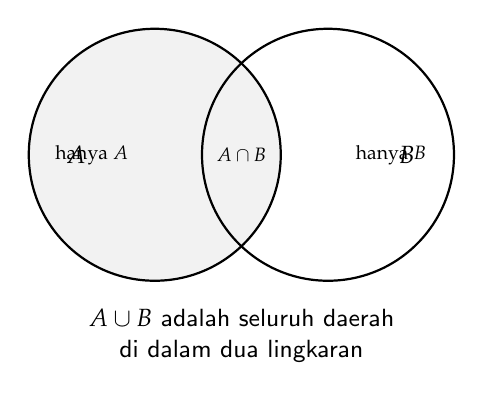
\begin{tikzpicture}[
			lbl/.style={font=\sffamily\small}
		]
		\draw[thick, fill=black!5] (0,0) circle (1.6);
		\draw[thick, fill=none] (2.2,0) circle (1.6);
		\node[lbl] at (-1.0,0) {$A$};
		\node[lbl] at (3.2,0) {$B$};
		\node[font=\scriptsize, align=center] at (-0.8,0) {hanya $A$};
		\node[font=\scriptsize, align=center] at (1.1,0) {$A \cap B$};
		\node[font=\scriptsize, align=center] at (3.0,0) {hanya $B$};
		\node[font=\small\sffamily, align=center] at (1.1,-2.3) {$A \cup B$ adalah seluruh daerah\\di dalam dua lingkaran};
	\end{tikzpicture}
	\caption{Irisan dan gabungan dua himpunan.}
	\label{fig:irisan-gabungan}
\end{figure}

Deskripsi tekstual Gambar~\ref{fig:irisan-gabungan}: dua lingkaran berpotongan. Lingkaran kiri adalah $A$, lingkaran kanan adalah $B$. Daerah tengah adalah $A \cap B$. Seluruh daerah di dalam kedua lingkaran adalah $A \cup B$. Daerah kiri saja adalah elemen $A$ yang bukan elemen $B$. Daerah kanan saja adalah elemen $B$ yang bukan elemen $A$.

\subsection{Selisih dan Beda Simetris}

Selisih $A-B$ berisi elemen $A$ yang bukan elemen $B$. Beda simetris $A \oplus B$ berisi elemen yang ada di $A$ atau di $B$, tetapi tidak di keduanya. Dalam basis data relasional, selisih setara dengan perintah EXCEPT atau NOT IN. Jika $A=\{\text{User1},\text{User2},\text{User3},\text{User5}\}$ adalah pengguna aktif dan $B=\{\text{User2},\text{User5}\}$ adalah pengguna yang sudah membayar, maka $A-B=\{\text{User1},\text{User3}\}$ adalah pengguna aktif yang belum membayar \cite{silberschatz}. Perhatikan Gambar~\ref{fig:selisih-simetris}.

\begin{figure}[H]
	\centering
	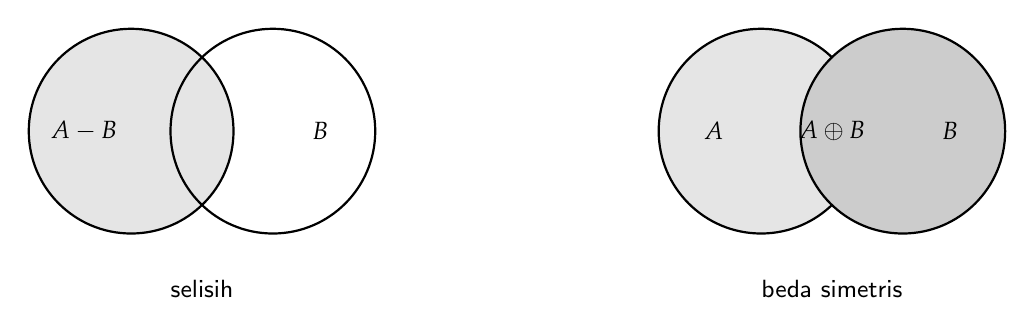
\begin{tikzpicture}[
			lbl/.style={font=\sffamily\small}
		]
		\begin{scope}[shift={(-4,0)}]
			\draw[thick, fill=black!10] (0,0) circle (1.3);
			\draw[thick, fill=none] (1.8,0) circle (1.3);
			\node[lbl] at (-0.6,0) {$A-B$};
			\node[lbl] at (2.4,0) {$B$};
			\node[font=\small\sffamily] at (0.9,-2) {selisih};
		\end{scope}
		\begin{scope}[shift={(4,0)}]
			\draw[thick, fill=black!10] (0,0) circle (1.3);
			\draw[thick, fill=black!20] (1.8,0) circle (1.3);
			\node[lbl] at (-0.6,0) {$A$};
			\node[lbl] at (2.4,0) {$B$};
			\node[lbl] at (0.9,0) {$A \oplus B$};
			\node[font=\small\sffamily] at (0.9,-2) {beda simetris};
		\end{scope}
	\end{tikzpicture}
	\caption{Selisih dan beda simetris dua himpunan.}
	\label{fig:selisih-simetris}
\end{figure}

Deskripsi tekstual Gambar~\ref{fig:selisih-simetris}: gambar kiri menunjukkan $A-B$, yaitu bagian lingkaran $A$ yang tidak beririsan dengan $B$. Gambar kanan menunjukkan $A \oplus B$, yaitu bagian kiri saja ditambah bagian kanan saja, tanpa daerah irisan.

\subsection{Produk Kartesian}

Produk kartesian $A \times B$ adalah himpunan semua pasangan berurutan $(a,b)$ dengan $a \in A$ dan $b \in B$. Jika $A=\{\text{Chrome},\text{Firefox}\}$ dan $B=\{\text{Windows},\text{Linux},\text{MacOS}\}$, maka $A \times B$ berisi enam pasangan. Dalam pengujian perangkat lunak, produk kartesian dipakai untuk menghasilkan kombinasi browser dan sistem operasi yang harus diuji \cite{silberschatz}. Perhatikan Gambar~\ref{fig:produk-kartesian}.

\begin{figure}[H]
	\centering
	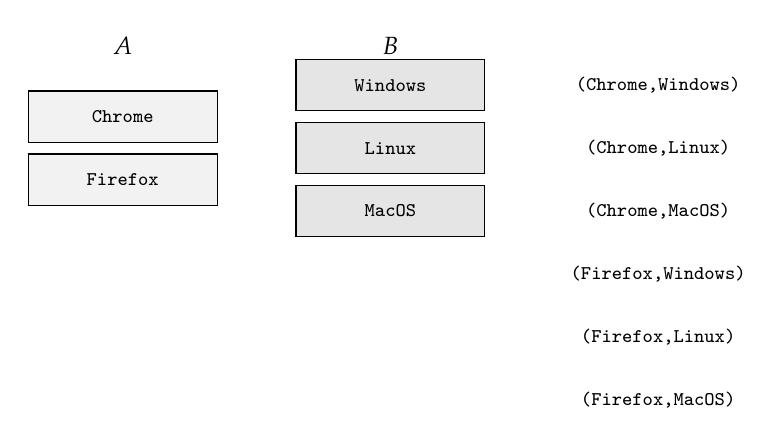
\begin{tikzpicture}[
			cell/.style={rectangle, draw=black, minimum width=2.4cm, minimum height=0.65cm, align=center, font=\ttfamily\scriptsize},
			hdr/.style={font=\sffamily\small}
		]
		\node[hdr] at (0,0.9) {$A$};
		\node[hdr] at (3.4,0.9) {$B$};
		\node[cell, fill=black!5] (a1) at (0,0) {Chrome};
		\node[cell, fill=black!5] (a2) at (0,-0.8) {Firefox};
		\node[cell, fill=black!10] (b1) at (3.4,0.4) {Windows};
		\node[cell, fill=black!10] (b2) at (3.4,-0.4) {Linux};
		\node[cell, fill=black!10] (b3) at (3.4,-1.2) {MacOS};
		\node[font=\ttfamily\scriptsize, align=left] at (6.8,0.4) {(Chrome,Windows)};
		\node[font=\ttfamily\scriptsize, align=left] at (6.8,-0.4) {(Chrome,Linux)};
		\node[font=\ttfamily\scriptsize, align=left] at (6.8,-1.2) {(Chrome,MacOS)};
		\node[font=\ttfamily\scriptsize, align=left] at (6.8,-2.0) {(Firefox,Windows)};
		\node[font=\ttfamily\scriptsize, align=left] at (6.8,-2.8) {(Firefox,Linux)};
		\node[font=\ttfamily\scriptsize, align=left] at (6.8,-3.6) {(Firefox,MacOS)};
	\end{tikzpicture}
	\caption{Produk kartesian browser dan sistem operasi.}
	\label{fig:produk-kartesian}
\end{figure}

Deskripsi tekstual Gambar~\ref{fig:produk-kartesian}: kolom kiri berisi dua browser, yaitu Chrome dan Firefox. Kolom tengah berisi tiga sistem operasi, yaitu Windows, Linux, dan MacOS. Kolom kanan berisi enam pasangan berurutan hasil produk kartesian. Setiap browser dipasangkan tepat satu kali dengan setiap sistem operasi.

\begin{table}[H]
	\centering
	\caption{Ringkasan operasi himpunan.}
	\label{tab:operasi-himpunan}
	\small
	\begin{tabularx}{\textwidth}{l l X}
		\toprule
		Operasi          & Notasi         & Makna                                            \\
		\midrule
		Irisan           & $A \cap B$     & elemen yang ada di $A$ dan $B$                   \\
		Gabungan         & $A \cup B$     & elemen yang ada di $A$ atau $B$                  \\
		Komplemen        & $\overline{A}$ & elemen semesta yang bukan elemen $A$             \\
		Selisih          & $A-B$          & elemen $A$ yang bukan elemen $B$                 \\
		Beda simetris    & $A \oplus B$   & elemen di salah satu himpunan, tidak di keduanya \\
		Produk kartesian & $A \times B$   & semua pasangan berurutan $(a,b)$                 \\
		\bottomrule
	\end{tabularx}
\end{table}

\section{Prinsip Inklusi-Eksklusi}

\subsection{Dua Himpunan}

Untuk dua himpunan berhingga, berlaku $|A \cup B|=|A|+|B|-|A \cap B|$. Contoh: $A$ adalah pengguna Mobile App dengan $|A|=3500$, $B$ adalah pengguna Web dengan $|B|=2100$, dan $|A \cap B|=800$. Maka $|A \cup B|=3500+2100-800=4800$ pengguna unik. Pengurangan irisan mencegah penghitungan ganda. Tanpa pengurangan itu, hasilnya menjadi 5600, yaitu terlalu besar sebesar 800 \cite{rosen}.

\subsection{Tiga Himpunan}

Untuk tiga himpunan, berlaku rumus $|N \cup D \cup V|=|N|+|D|+|V|-|N \cap D|-|N \cap V|-|D \cap V|+|N \cap D \cap V|$. Dengan data $|N|=120$, $|D|=80$, $|V|=60$, $|N \cap D|=40$, $|N \cap V|=25$, $|D \cap V|=15$, dan $|N \cap D \cap V|=10$, hasilnya adalah $120+80+60-40-25-15+10=190$. Perhatikan Gambar~\ref{fig:tiga-himpunan}.

\begin{figure}[H]
	\centering
	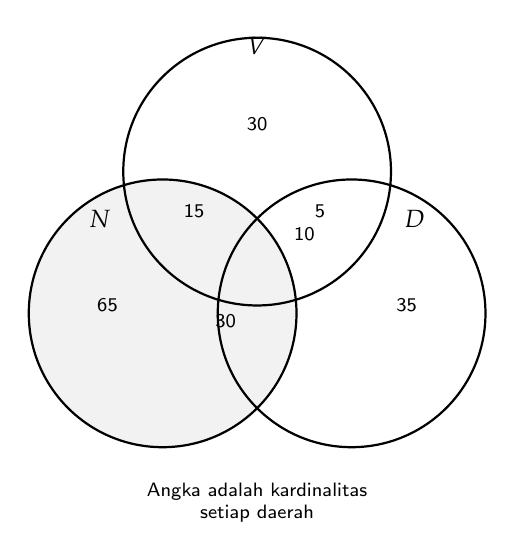
\begin{tikzpicture}[
			num/.style={font=\scriptsize\sffamily, align=center}
		]
		\draw[thick, fill=black!5] (0,0) circle (1.7);
		\draw[thick, fill=none] (2.4,0) circle (1.7);
		\draw[thick, fill=none] (1.2,1.8) circle (1.7);
		\node[font=\sffamily\small] at (-0.8,1.2) {$N$};
		\node[font=\sffamily\small] at (3.2,1.2) {$D$};
		\node[font=\sffamily\small] at (1.2,3.4) {$V$};
		\node[num] at (-0.7,0.1) {65};
		\node[num] at (3.1,0.1) {35};
		\node[num] at (1.2,2.4) {30};
		\node[num] at (0.8,-0.1) {30};
		\node[num] at (1.8,1.0) {10};
		\node[num] at (0.4,1.3) {15};
		\node[num] at (2.0,1.3) {5};
		\node[font=\scriptsize\sffamily, align=center] at (1.2,-2.4) {Angka adalah kardinalitas\\setiap daerah};
	\end{tikzpicture}
	\caption{Diagram inklusi-eksklusi tiga himpunan.}
	\label{fig:tiga-himpunan}
\end{figure}

Deskripsi tekstual Gambar~\ref{fig:tiga-himpunan}: tiga lingkaran berpotongan berlabel $N$, $D$, dan $V$. Daerah khusus $N$ berisi 65, daerah khusus $D$ berisi 35, dan daerah khusus $V$ berisi 30. Daerah $N \cap D$ saja berisi 30, $N \cap V$ saja berisi 15, dan $D \cap V$ saja berisi 5. Daerah irisan ketiganya berisi 10. Jika seluruh angka dijumlahkan, hasilnya 190, yaitu kardinalitas gabungan tiga himpunan.

\begin{table}[H]
	\centering
	\caption{Ringkasan prinsip inklusi-eksklusi.}
	\label{tab:inklusi}
	\small
	\begin{tabularx}{\textwidth}{l X}
		\toprule
		Kasus          & Rumus dan makna                                                                    \\
		\midrule
		Dua himpunan   & $|A \cup B|=|A|+|B|-|A \cap B|$                                                    \\
		Tiga himpunan  & $|A \cup B \cup C|=|A|+|B|+|C|-|A \cap B|-|A \cap C|-|B \cap C|+|A \cap B \cap C|$ \\
		Tujuan         & menghindari penghitungan ganda pada daerah irisan                                  \\
		Kesalahan umum & menjumlahkan semua kategori tanpa mengurangi irisan                                \\
		\bottomrule
	\end{tabularx}
\end{table}

\section{Himpunan Fuzzy}

\subsection{Crisp dan Fuzzy}

Himpunan crisp memakai keanggotaan biner. Nilai $\mu_A(x)$ hanya 0 atau 1. Himpunan fuzzy memakai derajat keanggotaan pada selang $[0,1]$. Nilai 0,7 berarti elemen cenderung kuat menjadi anggota, tetapi tidak mutlak. Himpunan fuzzy diperkenalkan oleh Zadeh untuk menangani ketidakpastian dan ekspresi linguistik seperti sedikit, lumayan, dan sangat \cite{zadeh}. Perhatikan Gambar~\ref{fig:crisp-fuzzy}.

\begin{figure}[H]
	\centering
	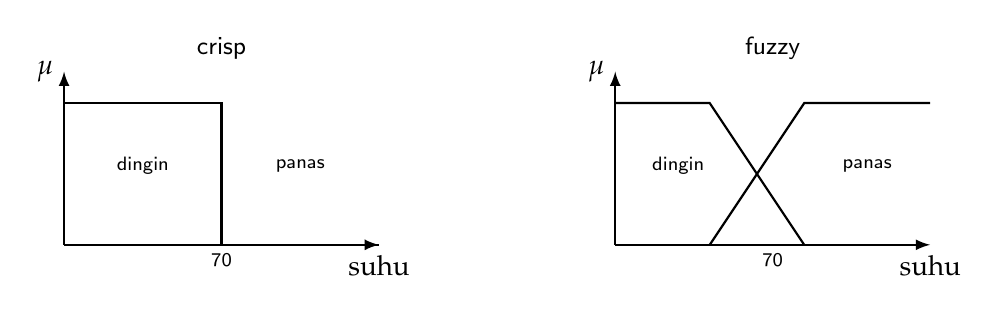
\begin{tikzpicture}[
			axis/.style={draw, thick, -latex},
			lbl/.style={font=\sffamily\small},
			tick/.style={font=\scriptsize\sffamily}
		]
		\begin{scope}[shift={(-4.5,0)}]
			\draw[axis] (0,0) -- (4,0) node[below] {suhu};
			\draw[axis] (0,0) -- (0,2.2) node[left] {$\mu$};
			\draw[thick] (0,1.8) -- (2,1.8) -- (2,0) -- (4,0);
			\node[tick] at (1,1.0) {dingin};
			\node[tick] at (3,1.0) {panas};
			\node[tick] at (2,-0.2) {70};
			\node[lbl] at (2,2.5) {crisp};
		\end{scope}
		\begin{scope}[shift={(2.5,0)}]
			\draw[axis] (0,0) -- (4,0) node[below] {suhu};
			\draw[axis] (0,0) -- (0,2.2) node[left] {$\mu$};
			\draw[thick] (0,1.8) -- (1.2,1.8) -- (2.4,0);
			\draw[thick] (1.2,0) -- (2.4,1.8) -- (4,1.8);
			\node[tick] at (0.8,1.0) {dingin};
			\node[tick] at (3.2,1.0) {panas};
			\node[tick] at (2,-0.2) {70};
			\node[lbl] at (2,2.5) {fuzzy};
		\end{scope}
	\end{tikzpicture}
	\caption{Perbandingan fungsi keanggotaan crisp dan fuzzy.}
	\label{fig:crisp-fuzzy}
\end{figure}

Deskripsi tekstual Gambar~\ref{fig:crisp-fuzzy}: grafik kiri adalah crisp. Pada suhu di bawah 70, nilai keanggotaan dingin adalah 1 dan panas adalah 0. Pada suhu 70 ke atas, nilai berubah mendadak. Grafik kanan adalah fuzzy. Nilai dingin menurun secara miring dan nilai panas meningkat secara miring. Pada suhu 70, kedua nilai berada di tengah, sehingga suhu itu dapat dianggap sebagian dingin dan sebagian panas.

\subsection{Fungsi Keanggotaan Fuzzy}

Fungsi keanggotaan fuzzy memetakan elemen ke nilai pada $[0,1]$. Jika himpunan usia memiliki kategori MUDA, PAROBAYA, dan TUA, maka usia 40 dapat memiliki $\mu_{\text{MUDA}}(40)=0{,}25$ dan $\mu_{\text{PAROBAYA}}(40)=0{,}50$. Artinya, usia 40 lebih condong ke PAROBAYA daripada MUDA, tetapi masih memiliki derajat MUDA. Perhatikan Gambar~\ref{fig:usia-fuzzy}.

\begin{figure}[H]
	\centering
	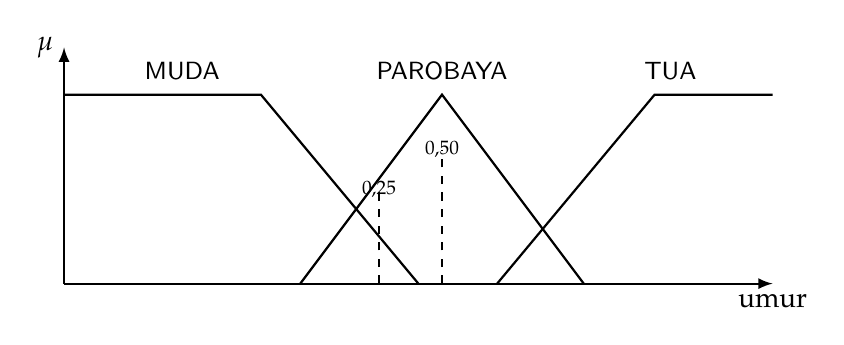
\begin{tikzpicture}[
			axis/.style={draw, thick, -latex},
			lbl/.style={font=\sffamily\small}
		]
		\draw[axis] (0,0) -- (9,0) node[below] {umur};
		\draw[axis] (0,0) -- (0,3) node[left] {$\mu$};
		\draw[thick] (0,2.4) -- (2.5,2.4) -- (4.5,0);
		\draw[thick] (3,0) -- (4.8,2.4) -- (6.6,0);
		\draw[thick] (5.5,0) -- (7.5,2.4) -- (9,2.4);
		\node[lbl] at (1.5,2.7) {MUDA};
		\node[lbl] at (4.8,2.7) {PAROBAYA};
		\node[lbl] at (7.7,2.7) {TUA};
		\node[font=\scriptsize\sffamily] at (4.0,1.2) {$0{,}25$};
		\node[font=\scriptsize\sffamily] at (4.8,1.7) {$0{,}50$};
		\draw[dashed] (4.0,0) -- (4.0,1.2);
		\draw[dashed] (4.8,0) -- (4.8,1.7);
	\end{tikzpicture}
	\caption{Fungsi keanggotaan fuzzy untuk kategori usia.}
	\label{fig:usia-fuzzy}
\end{figure}

Deskripsi tekstual Gambar~\ref{fig:usia-fuzzy}: tiga kurva segitiga dan trapesium mewakili MUDA, PAROBAYA, dan TUA. Garis putus-putus pada usia 40 menunjukkan nilai keanggotaan MUDA sebesar 0,25 dan PAROBAYA sebesar 0,50. Semakin tinggi nilai keanggotaan, semakin kuat elemen itu masuk ke kategori tersebut.

\subsection{Contoh Peringkat Rekomendasi}

Jika Film A memiliki derajat suka 0,7, Film B memiliki derajat netral 0,5, dan Film C memiliki derajat suka sangat 1, maka urutan rekomendasi dari paling disukai adalah Film C, Film A, lalu Film B. Himpunan fuzzy lebih tepat daripada himpunan crisp karena preferensi pengguna tidak selalu ya atau tidak. Nilai 0,7 dan 0,5 memberi urutan yang lebih kaya daripada hanya suka dan tidak suka \cite{zadeh}. Ringkasan perbandingan crisp dan fuzzy diberikan pada Tabel~\ref{tab:crisp-fuzzy}.

\begin{table}[H]
	\centering
	\caption{Perbandingan himpunan crisp dan fuzzy.}
	\label{tab:crisp-fuzzy}
	\small
	\begin{tabularx}{\textwidth}{l X X}
		\toprule
		Aspek              & Crisp                & Fuzzy                              \\
		\midrule
		Nilai keanggotaan  & 0 atau 1             & bilangan real pada $[0,1]$         \\
		Batas kategori     & tegas                & bertahap                           \\
		Contoh suhu        & dingin atau panas    & sebagian dingin dan sebagian panas \\
		Contoh rekomendasi & suka atau tidak suka & derajat suka 0,7                   \\
		Kegunaan           & aturan biner         & penilaian bertingkat               \\
		\bottomrule
	\end{tabularx}
\end{table}

\section{Perbandingan dan Sintesis}

Tabel~\ref{tab:sintesis} menyandingkan konsep utama dalam satu pandangan. Kolom pertama menyebut lapisan konsep. Kolom kedua menyebut pertanyaan yang dijawab. Kolom ketiga menyebut alat matematis. Kolom keempat menyebut contoh penerapan.

\begin{table}[H]
	\centering
	\caption{Sintesis konsep himpunan untuk rekayasa perangkat lunak.}
	\label{tab:sintesis}
	\footnotesize
	\begin{tabularx}{\textwidth}{l X X X}
		\toprule
		Lapisan        & Pertanyaan                                       & Alat                             & Contoh penerapan        \\
		\midrule
		Dasar          & apa saja anggota kumpulan ini                    & notasi himpunan dan kardinalitas & daftar pengguna unik    \\
		Relasi         & apakah satu kumpulan bagian dari kumpulan lain   & subset dan superset              & hierarki hak akses      \\
		Operasi        & bagaimana menggabungkan atau memisahkan kumpulan & irisan, gabungan, selisih        & filter pengguna aktif   \\
		Hitung         & berapa total unik tanpa penghitungan ganda       & inklusi-eksklusi                 & pengguna Mobile dan Web \\
		Ketidakpastian & seberapa kuat elemen masuk kategori              & himpunan fuzzy                   & skor rekomendasi film   \\
		\bottomrule
	\end{tabularx}
\end{table}

Sintesis dari Tabel~\ref{tab:sintesis} adalah satu pola berpikir. Data mentah diubah menjadi himpunan unik, lalu himpunan itu dioperasikan, lalu dihitung dengan koreksi irisan, dan jika perlu diberi derajat keanggotaan fuzzy. Pola ini berlaku dari analitik pengguna sampai sistem rekomendasi.

\section{Studi Kasus: Dashboard Pengguna E-commerce}

\subsection{Langkah 1: Kumpulkan Data Mentah}

Data yang tersedia adalah 10.000 pengguna, 6.000 pengguna Mobile App, 4.500 pengguna Web, 2.000 pengguna keduanya, 5.500 pengguna melakukan pembelian, dan 1.500 pengguna memakai Mobile App dan Web serta melakukan pembelian. Data mentah ini belum menjadi informasi karena batas antar kategori belum dinyatakan sebagai himpunan.

\subsection{Langkah 2: Bentuk Himpunan Pengguna Unik}

Bentuk $M$ sebagai himpunan pengguna Mobile App, $W$ sebagai himpunan pengguna Web, dan $P$ sebagai himpunan pengguna yang melakukan pembelian. Kardinalitasnya adalah $|M|=6000$, $|W|=4500$, $|P|=5500$, dan $|M \cap W|=2000$. Himpunan menghapus duplikat sehingga satu pengguna yang membuka aplikasi tiga kali tetap dihitung satu.

\subsection{Langkah 3: Definisikan Semesta Pembicaraan}

Semesta $U$ adalah seluruh pengguna yang tercatat pada periode analisis. Tanpa semesta, komplemen tidak dapat dihitung. Jika $U$ adalah 10.000 pengguna, maka pengguna yang tidak memakai Mobile App dan tidak memakai Web adalah komplemen dari $M \cup W$. Namun nilai itu baru sah jika $U$ benar-benar memuat semua pengguna yang relevan.

\subsection{Langkah 4: Hitung Irisan}

Irisan $M \cap W$ berisi pengguna yang memakai Mobile App dan Web. Nilainya diketahui 2.000. Angka ini menjadi koreksi utama karena pengguna di daerah itu akan dihitung dua kali jika $|M|$ dan $|W|$ dijumlahkan langsung.

\subsection{Langkah 5: Hitung Gabungan}

Gabungan $M \cup W$ berisi pengguna yang memakai salah satu atau kedua platform. Dengan inklusi-eksklusi, $|M \cup W|=6000+4500-2000=8500$. Jadi ada 8.500 pengguna unik yang memakai Mobile App atau Web.

\subsection{Langkah 6: Hitung Daerah Khusus}

Pengguna hanya Mobile App adalah $|M-W|=|M|-|M \cap W|=6000-2000=4000$. Pengguna hanya Web adalah $|W-M|=|W|-|M \cap W|=4500-2000=2500$. Kedua angka ini menjawab pertanyaan dashboard tentang komposisi pengguna per platform.

\subsection{Langkah 7: Hitung Beda Simetris}

Pengguna yang memakai Mobile App atau Web tetapi tidak keduanya adalah $|M \oplus W|=|M \cup W|-|M \cap W|=8500-2000=6500$. Angka ini juga sama dengan $4000+2500=6500$. Beda simetris berguna untuk kampanye yang menyasar pengguna yang baru memakai satu platform.

\subsection{Langkah 8: Periksa Kelengkapan Data Tiga Himpunan}

Untuk menghitung $|M \cup W \cup P|$, diperlukan $|M \cap P|$ dan $|W \cap P|$. Data yang tersedia hanya $|M \cap W \cap P|=1500$. Jadi dashboard belum boleh menampilkan gabungan tiga himpunan secara final. Langkah yang benar adalah menandai data yang kurang, bukan mengarang angka. Inilah sikap akademik yang diuji oleh kasus ini \cite{silberschatz}. Alur langkah studi kasus ditunjukkan pada Gambar~\ref{fig:alur-studi-kasus}.

\begin{figure}[H]
	\centering
	\begin{tikzpicture}[
			step/.style={rectangle, draw=black, thick, fill=black!5, text width=9cm, align=left, minimum height=0.7cm, font=\sffamily\small, inner sep=8pt},
			line/.style={draw, thick, -latex}
		]
		\node[step] (s1) {\textbf{1.} Kumpulkan log aktivitas};
		\node[step, below=0.25cm of s1] (s2) {\textbf{2.} Bentuk himpunan pengguna unik};
		\node[step, below=0.25cm of s2] (s3) {\textbf{3.} Definisikan $M$, $W$, dan $P$};
		\node[step, below=0.25cm of s3] (s4) {\textbf{4.} Hitung irisan dan gabungan};
		\node[step, below=0.25cm of s4] (s5) {\textbf{5.} Hitung daerah khusus};
		\node[step, below=0.25cm of s5] (s6) {\textbf{6.} Hitung beda simetris};
		\node[step, below=0.25cm of s6] (s7) {\textbf{7.} Periksa irisan dengan $P$};
		\node[step, below=0.25cm of s7] (s8) {\textbf{8.} Susun dashboard};
		\draw[line] (s1) -- (s2);
		\draw[line] (s2) -- (s3);
		\draw[line] (s3) -- (s4);
		\draw[line] (s4) -- (s5);
		\draw[line] (s5) -- (s6);
		\draw[line] (s6) -- (s7);
		\draw[line] (s7) -- (s8);
	\end{tikzpicture}
	\caption{Alur delapan langkah studi kasus dashboard pengguna.}
	\label{fig:alur-studi-kasus}
\end{figure}

Deskripsi tekstual Gambar~\ref{fig:alur-studi-kasus}: delapan kotak bertumpuk dari atas ke bawah. Setiap kotak berisi satu langkah. Panah mengarah ke kotak berikutnya. Urutan dimulai dari pengumpulan log, pembentukan himpunan unik, definisi tiga himpunan, perhitungan irisan dan gabungan, perhitungan daerah khusus, perhitungan beda simetris, pemeriksaan kelengkapan data, dan diakhiri penyusunan dashboard.

\begin{table}[H]
	\centering
	\caption{Ringkasan hasil studi kasus dashboard pengguna.}
	\label{tab:studi-kasus}
	\small
	\begin{tabularx}{\textwidth}{l X l}
		\toprule
		Langkah & Operasi                    & Hasil                              \\
		\midrule
		1       & data mentah                & 10.000 pengguna                    \\
		2       & bentuk $M$, $W$, $P$       & $|M|=6000$, $|W|=4500$, $|P|=5500$ \\
		3       & irisan $M \cap W$          & 2.000                              \\
		4       & gabungan $M \cup W$        & 8.500                              \\
		5       & hanya Mobile               & 4.000                              \\
		6       & hanya Web                  & 2.500                              \\
		7       & beda simetris $M \oplus W$ & 6.500                              \\
		8       & gabungan tiga himpunan     & belum final karena data kurang     \\
		\bottomrule
	\end{tabularx}
\end{table}

\section{Kesalahan Umum dan Cara Menghindarinya}

Tabel~\ref{tab:kesalahan} memuat kesalahan yang paling sering muncul saat memakai teori himpunan dalam analisis data.

\begin{table}[H]
	\centering
	\caption{Kesalahan umum pada penerapan teori himpunan.}
	\label{tab:kesalahan}
	\footnotesize
	\begin{tabularx}{\textwidth}{l X X}
		\toprule
		Kesalahan                                & Akibat                    & Perbaikan                             \\
		\midrule
		menghitung larik mentah sebagai himpunan & duplikat ikut terhitung   & bentuk himpunan unik lebih dahulu     \\
		menjumlahkan $|A|+|B|$ tanpa irisan      & hasil terlalu besar       & kurangi $|A \cap B|$                  \\
		menganggap subset sama dengan elemen     & relasi salah              & bedakan $x \in A$ dan $A \subseteq B$ \\
		lupa mendefinisikan semesta              & komplemen tidak sah       & tulis $U$ secara eksplisit            \\
		mencampur notasi crisp dan fuzzy         & makna nilai kabur         & tetapkan domain nilai keanggotaan     \\
		menghitung $|P(A)|=n$                    & hasil salah               & gunakan $2^n$                         \\
		mengabaikan data irisan tiga himpunan    & gabungan tidak final      & tandai data yang kurang               \\
		memakai warna untuk membedakan daerah    & tidak terbaca hitam-putih & pakai label dan gradasi abu-abu       \\
		menulis $A-B$ sebagai $B-A$              & arah selisih salah        & periksa elemen mana yang dikurangi    \\
		\bottomrule
	\end{tabularx}
\end{table}

Dua kesalahan yang paling sering adalah menjumlahkan kategori tanpa koreksi irisan dan melupakan semesta pembicaraan. Kesalahan pertama membuat dashboard terlalu optimistis. Kesalahan kedua membuat komplemen menjadi tidak bermakna. Keduanya dapat dicegah dengan menulis definisi himpunan sebelum menghitung.

\section{Lembar Rujukan Cepat}

Tabel~\ref{tab:rujukan-cepat} adalah lembar rujukan untuk ujian atau kerja.

\begin{table}[H]
	\centering
	\caption{Lembar rujukan cepat teori himpunan.}
	\label{tab:rujukan-cepat}
	\footnotesize
	\begin{tabularx}{\textwidth}{l X}
		\toprule
		Kebutuhan                      & Notasi atau langkah                                                                \\
		\midrule
		menyatakan elemen              & $x \in A$                                                                          \\
		menyatakan bukan elemen        & $x \notin A$                                                                       \\
		menulis himpunan               & $A=\{a,b,c\}$                                                                      \\
		menulis aturan                 & $A=\{x \mid \text{syarat}\}$                                                       \\
		kardinalitas                   & $|A|$                                                                              \\
		himpunan kosong                & $\varnothing$                                                                      \\
		subset                         & $A \subseteq B$                                                                    \\
		superset                       & $B \supseteq A$                                                                    \\
		himpunan kuasa                 & $P(A)$ dan $|P(A)|=2^{|A|}$                                                        \\
		irisan                         & $A \cap B$                                                                         \\
		gabungan                       & $A \cup B$                                                                         \\
		komplemen                      & $\overline{A}$                                                                     \\
		selisih                        & $A-B$                                                                              \\
		beda simetris                  & $A \oplus B$                                                                       \\
		produk kartesian               & $A \times B$                                                                       \\
		inklusi-eksklusi dua himpunan  & $|A \cup B|=|A|+|B|-|A \cap B|$                                                    \\
		inklusi-eksklusi tiga himpunan & $|A \cup B \cup C|=|A|+|B|+|C|-|A \cap B|-|A \cap C|-|B \cap C|+|A \cap B \cap C|$ \\
		keanggotaan fuzzy              & $\mu_A(x) \in [0,1]$                                                               \\
		\bottomrule
	\end{tabularx}
\end{table}

\section{Kesimpulan}

Modul ini menunjukkan bahwa teori himpunan bukan bahan hafalan, melainkan alat kerja. Tiga prinsip penutup adalah sebagai berikut.

\begin{enumerate}
	\item Nyatakan batas himpunan sebelum menghitung. Tanpa definisi yang jelas, angka apa pun bisa tampak benar.
	\item Koreksi irisan sebelum menjumlahkan. Prinsip inklusi-eksklusi mencegah penghitungan ganda.
	\item Gunakan derajat keanggotaan ketika data tidak biner. Himpunan fuzzy memberi urutan yang lebih jujur daripada kategori ya atau tidak.
\end{enumerate}

Dengan tiga prinsip itu, pembaca dapat berpindah dari data mentah menuju dashboard yang dapat dipertanggungjawabkan, serta siap mempelajari topik berikutnya dalam seri matematika diskrit.

\newpage
\section*{Referensi}
\addcontentsline{toc}{section}{Referensi}

\begin{thebibliography}{99}

	\bibitem{rosen}
	Rosen, K. H. (2019).
	\textit{Discrete Mathematics and Its Applications} (8th ed.).
	McGraw-Hill Education.

	\bibitem{munir}
	Munir, R. (2012).
	\textit{Matematika Diskrit}.
	Informatika.

	\bibitem{epp}
	Epp, S. S. (2010).
	\textit{Discrete Mathematics with Applications} (4th ed.).
	Brooks Cole.

	\bibitem{lipschutz}
	Lipschutz, S., \& Lipson, M. (2007).
	\textit{Discrete Mathematics}.
	McGraw-Hill.

	\bibitem{zadeh}
	Zadeh, L. A. (1965).
	Fuzzy Sets.
	\textit{Information and Control}, 8(3), 338--353.

	\bibitem{silberschatz}
	Silberschatz, A., Korth, H. F., \& Sudarshan, S. (2019).
	\textit{Database System Concepts} (7th ed.).
	McGraw-Hill Education.

	\bibitem{kleppmann}
	Kleppmann, M. (2017).
	\textit{Designing Data-Intensive Applications}.
	O'Reilly Media.

	\bibitem{sommerville}
	Sommerville, I. (2016).
	\textit{Software Engineering} (10th ed.).
	Pearson.

\end{thebibliography}

\end{document}
